% !TEX root = ../../main.tex

We have previously seen the challenges of edge computing architectures
and the requirements to fulfill collaborative applications needs.
We will now study the state of the art of edge storage systems from
a set of examples.
We will cover the spectrum of fog computing systems from cloud geo-distributed 
approaches to decentralized edge systems, 
and assess the strengths and weaknesses of these approaches
in terms of consistency, availability, mobility and security.
We will also see more distant related work,
with fully decentralized web and mobile oriented systems.


\section{Overview}

Much previous work on data in edge computing 
\cite{app:rep:1826, syn:optim:rep:1433, rep:1844}
focuses on streaming and content delivery.

Examples include sensor systems or propagating database views.
We leverage this previous work by propagating shared state as a
stream of update events.
The distributed sharing of persistent mutable state raises extra
challenges, which we address in this state of the art study.

Achieving low response time is an ongoing challenge for many web applications
\cite{akamai:2010:press, kohavi2007online, leighton2009improving}.
For example, on amazon.com, a delay of 100 ms costs in average 1\% of
sales \cite{kohavi2007online}.
In order to deliver fast response and offline support, a number of web
applications cache data at the client side, e.g., in the browser.
See for instance Facebook's News Feed \cite{facebook:newsfeed}, or the
Chrome browser extension that enables Google Docs and Google Maps to be
used offline \cite{googledocs:offline}.
Several earlier systems manage data for clients that are connected only
intermittently \cite{optim:rep:syn:1500,rep:syn:app:1728}.
Bayou \cite{syn:optim:rep:1433} supports data replicas in
mobile computers.
Cimbiosys \cite{app:rep:1826} uses a decentralized model to support
Internet Services.

Rover \cite{rep:1844} and Coda \cite{fic:rep:887} are general-purpose
systems that support disconnected operation, under a weak consistency
model.


Cloud Types \cite{syn:app:1761} support a programming
model for shared cloud data, similar to CRDTs with total order.
It supports multiple replicas of data, synchronized periodically.
Parse \cite{syn:app:1761} is similar, under a weaker eventual consistency
model.

% CC, CC+ and TCC+
Strengthening causal consistency with strong convergence was proposed by
COPS under the name Causal Plus Consistency (CC+) \cite{rep:syn:1662}.
ChainReaction augments CC+ with transactional reads, implemented with
the help of a sequencer per DC.
To execute a write, ChainReaction requires that the prior versions read at the client are stable in the DC.
%
TCC+ \cite{rep:pro:sh182} extends the guarantees of CC+ to transactions.
This model is closely related to others, such as Parallel Snapshot
Isolation (PSI) proposed by the Walter system \cite{rep:syn:1661}.
TCC+ is the strongest model compatible with availability under partition.
%It does order concurrent transactions, but only requires convergence.
\system{} guarantees TCC+ globally; in zones with good connectivity,
it enforces an SI zone to
improve metadata overhead and user experience.
Whereas TCC+ supports concurrent updates and arbitrary CRDT types, PSI
restricts concurrency to a single data type (the cset).
Its SI zones, the DCs, are fixed in advance.
Walter runs two-phase commit across data centers; this ensures global
transactions are strongly consistent, but negatively impacts liveliness
and performance.

% hybrid consistency models
A hybrid consistency model makes different consistency guarantees for
different operations.
For instance, in Lazy Replication, operations are causally consistent by
default, but can optionally request linearisability \cite{pan:rep:1146}.
References
\citealp{alg:rep:syn:optim:1464,rep:syn:sh167} or \citealp{rep:syn:1690}
are other examples.
%
Unistore \cite{unistore} supports both causal and linearisable
transactions over a geo-replicated key-value store.
To ensure fault tolerance, Unistore requires that, before a linearisable
transaction commits, all of its causal dependencies be stable.
%
\citet{fisheye} propose a proximity-based hybrid model, called Fisheye
Consistency, such that nodes that are close in a ``proximity graph''
mutually observe strongly-consistent transactions, whereas consistency
is weak between far-away nodes.

Depot \cite{rep:1712} and PRACTI \cite{rep:syn:1729} pioneered
highly available caching at the edge, under causal consistency.
Their approach uses vector clocks with one entry per replica, which severely
limits scalability.
Depot targets Byzantine fault tolerance, the most general class of
faults, but not transactions.
Simba \cite{fic:syn:1731} enables the edge application to select among a
specific level of consistency (eventual, causal or serialisable).
PouchDB \cite{pouchDB} is a client-side cache that replicates data
from a CouchDB server; it supports offline operation and detects
conflicts, but does not merge them.

SwiftCloud \cite{rep:pan:sh177} introduces bounded-size
vectors and migration.
Legion \cite{app:rep:syn:1775} is a web framework that extends applications
with peer-to-peer interaction using CRDTs.
\system{} is inspired by the above designs; additionally, \system{}
supports collaboration groups and peer groups, and ensures that
migration is seamless.

Let's study in detail each of these systems.

\section{Kronos}
\label{sec:soa:kronos}
Kronos \cite{escriva2014kronos} 
is a centralized service that maintains a dependency graph. 
Nodes represent events and edges define causal relationships between events. 

When a  client wants to obtain a reference to an event, 
he or she must contact Kronos. 
A reference is an identifier of an event and is managed by the service. 
After collecting a set of references,  clients need to know a possible order 
to apply the associated events. They must therefore contact Kronos, 
providing the set as input. 
The output is a sequence with all elements of the set that does not violate 
causality. 
Different clients may get different results, 
because the concurrent operations may be in a different order. 

Adding events to the graph is also done in two phases. 
In the first one, a client creates the event, receiving its reference. 
Then, it is able to assign an order, using the new event reference with the 
other existing references. There are two ways to order events: must and prefer. 
Must specify a strict order: either all must condition of a call is met, 
or the operation is aborted. The preferential order is used to assign 
relationships between concurrent operations. Its validity is checked only 
after Kronos has analyzed the must conditions. 
If they introduce inconsistencies, the operation is not aborted, 
but the order is rejected. Since this is not a geo-replicated solution, 
there are no remote servers to send new updates. 
This contributes to a simpler design, but creates a performance bottleneck. 

Kronos is an isolated system that deals only with the causality of events. 
This introduces a new abstraction, as different events can have very different 
granularities. 

The biggest weakness is related to how clients get a correct 
ordering of events. If a client has not received a reference that depends on 
another one that has been sent to the server, the ordering will create an 
inconsistent client state. So either the client must have all references to get 
a global order, 
or there must be an application-dependent protocol to prevent this. 

Despite an interesting approach to ensuring causal consistency, 
Kronos cannot be deployed at the edge. It is a centralized service 
that would quickly become a bottleneck, violating the scalability requirement.

\section{CloudPath}
\label{sec:soa:cloudpath}

CloudPath \cite{mortazavi2017cloudpath} provides a more 
general extension of possibly coherent storage systems to the network edge, 
while adding processing capabilities. It uses path computing to deploy a 
multi-tiered hierarchy from a data center to the edge node. 
As nodes get closer to end users, their performance gradually decreases. 
Overall, CloudPath connects three types of nodes in a tree structure: 
edge nodes (closest to end users), 
cloud nodes (most resource-rich and farthest away) and 
core nodes (any node in between). 
The root node replicates each object, 
while each descendant stores a subset of the items available in its parent. 
Clients read from and write to their local replicas, which propagate changes 
in the background through the hierarchy. If a client tries to read data that 
is not available locally, the node redirects the request to its parent and, 
until the data is found, the request moves up through the nodes. 
When there is a response, it follows the reverse path, causing each contacted 
child to store the new data. This creates on-demand data replication, 
attempting to cache only the latest requests. Updates are recorded in a write 
log with a label that contains the time of the change and the node ID. 
As a fault tolerance measure, updates are marked as dirty or clear. 
Dirty updates are not recognized by the parent node, but clear updates are 
replicated to both.

\section{COPS}
\label{sec:soa:cops}

COPS \cite{lloyd2011don} has a timestamp with one part per object. 
Each part has a logical clock. 

Clients are in charge of managing their causal history. 
In COPS, this history is called a context. 
Every time a client reads a new object, it adds the version to the context. 
The data center servers always give the latest consistent version of the object,
without looking at the client's context. 

When a client wants to write an object, 
it first uses the context to calculate the closest dependencies. 
The context can be seen as a dependency graph and the transitivity rule is 
used to find these dependencies. 
The closest dependency is obtained when one version of an object does not occur 
before another version. 
Then the client sends the object key, 
its new value and the closest dependencies to the local server. 
This server has all the dependencies, 
because the client maintains a session with it. 
It can therefore apply the update immediately, 
marking it with the dependencies and the new timestamp. 
This timestamp is sent back to the client and replaces all previous context. 

The remote update protocol follows similar steps as the local client update. 
When a server receives an object from another replica, 
it must check if the dependencies are met. 
Unlike the previous situation, 
there may be other updates that belong to the dependencies and are not yet 
present. 
Thus, the receiver must delay the update until it can be safely applied. 

An interesting feature is that a client can have different contexts for the 
same connection to the server. 
Since dependencies are tracked per client context, 
this allows independent operations to have fewer common dependencies, 
which reduces the time that remote updates wait before being visible 
(visibility latency). 

The timestamp format introduces some metadata compression, 
visible by having only one scalar per object and not a vector with one entry 
per replica. 
This results in a similar amount of metadata as Kronos, 
but with higher visibility latency. 

COPS was one of the first systems to provide causal consistency over cloud 
storage. 
However, the metadata format is not prepared for the size of the network edge. 
Typically, application workloads tend to include many more reads than writes. 
In this solution, the processing power required to check for remote update 
dependencies could overwhelm the nodes. 
In addition, it does not account for partial replication, 
as it was not a concern at the time.

\section{Orbe}
\label{sec:soa:orbe}

This system \cite{du2013orbe}
explores the layout of the data center to choose the number of 
timestamp partitions. 
Each data center is divided into N partitions and there are M different 
replicas. 
Considering that each partition is assigned to a different server, 
it is possible to address it through a matrix-like structure with N rows and M 
columns. 
Clients track their causal history with a copy of this matrix. 
It is filled with the logical clock of the corresponding server. 

A read-only client sends the key of the object. 
The server responds with the value of the last available version, 
the creation clock, 
and the index of the replica. 
If the entry pointed to by the index has a smaller value than the returned 
clock, 
then the client overwrites that position with the most recent value. 

To write an object, a client sends the key, 
the new value and its matrix to the local server responsible for the partition. 
The matrix corresponds to the update dependencies and is used during 
replication. 
Before marking the creation time, 
the server must increment its local clock, 
thus ensuring that the assigned value is unique. 
After storing the value and the object's metadata, 
the server responds with the update clock and its index. 
As with COPS, the client resets its causal history to default values, 
saving only the clock returned at the given index. 

To replicate updates, 
each partition communicates with its peers in different data centers. 
Updates are sent in order of creation with all associated information 
(key, value, creation clock, dependency matrix and replica index). 
To track the applied remote updates, 
there is a vector with one entry per replica and it contains the clocks of the 
last updates of each replica. 
The receiving server uses the matrix and the vector to check for dependencies. 
For its partition, 
it looks at the corresponding row of the same replicas and compares it to the 
vector. 
If the vector is greater than or equal to the row, 
the server can proceed to the next step. 
For other partitions, 
whenever there is a non-default value in the partition column, 
it means that the operation depends on other elements that the current data 
center may not store. 
So, the server contacts the servers that are in this situation, 
performing an explicit dependency check. 
If they fulfill the dependencies, 
the remote update can be made visible and the corresponding vector entry 
updated. 

In an effort to reduce the amount of metadata, 
the authors store only those matrix entries that are different from the default.
This strategy allows clients to store only the clocks of the contacted servers 
as dependencies for future operations. 
However, as soon as a client reads a newer version of a server, 
the matrix must be updated in the corresponding entry. 
This can lead to a matrix with all entries filled, 
which brings no gain in the worst case. 

Given the coarser grain in which dependencies are tracked, 
the impact of false dependencies will be greater. 
For example, updates on one server will depend on all previous updates applied 
on the same server. 
So even if there is no direct version dependency between objects, 
it will be treated as such. 
The increased wait time before updates can be applied will immediately result 
in higher visibility latency. 

Although Orbe is able to limit the size of metadata, 
it is not independent of the number of participants. 
Like COPS, Orbe requires replicas with full system state. 
Both of these features would not work at the network edge.

\section{PRACTI}
\label{sec:soa:practi}

The name of this system \cite{belaramani2006practi} includes its main features: partial replication (PR), arbitrary consistency (AC), and topological independence (TI). The granularity of partial replication is the finest, as each replica chooses the individual objects it wants to store. Like Orb, timestamping has one part per server and uses logical clocks. 

When a node wants to participate in the network, it chooses three sets of other nodes: one to receive updates, one to pick objects for its set of interest, and one to request more recent consistent versions of locally stored objects. The interest set is any group of objects that the node stores, and it can have one or more interest sets. 

Each node stores a global timestamp and as many timestamps as interest sets. They are updated at different times, expressing different things. They will be discussed when we talk about replicating updates. 

Nodes read their local copy of the object when it is valid. Validity is checked on timestamps and will be explained on update replication. 

Like reads, writes are performed on the local replica. Each version is tagged with the node's logical clock value. Then it is sent to the nodes that have subscribed to the object updates. 

The replication of updates is done by two types of messages: invalidations and bodies. The first type contains only metadata and can be precise (one message per object) or imprecise (one message for a group of objects and/or multiple updates), but must follow a causal delivery order. Imprecise messages have a set of targets, start and end clocks. Bodies have precise metadata and the actual data, and they do not need a specific delivery order. 

Upon receipt of invalidation messages, the node can update the timestamp of the object's interest set as well as that of the local node. The former is only updated with specific invalidations, but the latter joins the two. When the latter has a newer version, the local state is inaccurate. If the body for a specific invalidation has not yet arrived, the community of interest state is invalid. Invalid objects cannot be read, as this prevents inconsistencies for stronger models. However, for causal consistency, old values can be returned, which means that stale reads exist. 

Supporting different levels of consistency has an impact on the amount of metadata and the time needed to apply each update. Since all other systems are defined only for causal consistency, this will not be considered a negative feature. 

Although nodes can choose to keep only a subset of all existing objects, they must receive all invalidation messages. This is necessary because of the unstructured topology, which could otherwise lead to inconsistent information about the nodes. To reduce the impact of communication overhead, inaccurate invalidations function as a summary of updates whose data is not stored locally. Yet, nodes receive information about objects that they do not replicate, creating inauthentic partial replication. If all messages were about replicated objects, then this would be authentic partial replication. 

PRACTI is the first system to reveal some promising strategies that could be used for edge computing. Topology independence is particularly interesting because new nodes do not need to be integrated into a rigid structure using a join protocol. In addition, partial replication is supported, allowing machines with less storage to participate. However, metadata grows with the number of replicas, which could become unsustainable at the edge.

\section{Lazy Replication}
\label{sec:soa:lazy-replication}

Each node has full data replication, which means it must store all objects in the system. As in PRACTI, there is no predefined network topology and timestamps have a per-node portion. 

In lazy replication \cite{ladin1992providing}, there are two types of timestamps: unique identifiers (UIDs) and tags. The former marks updates and the latter compresses multiple UIDs. Tags create the client's causal history and dependencies for all operations. Servers also keep timestamps to track their current version. 

When reading the value of an object, the client sends the key and its label. The server waits for its state to include the entire history of the client. The response contains the last value of the object and the corresponding timestamp. Before delivering the value, the client updates its label by including the partial maximum between its previous label and the received timestamp. 

When a client tries to write an object, it constantly contacts the known entities by sending the object key, the new value and its label. Eventually it may send it to different entities and create duplicates. Given the desire to deliver messages at least once, each client has its client identifier (CID). It is included in the other update metadata, allowing different replicas to recognize duplicate updates. On the server side, if it is a new update, it increments its clock, updating its local label. The UID of the update is obtained by replacing the client label part of the local server with the new clock value. In response, the server sends the update UID, which is able to replace the client label while maintaining the causal history. Finally, the client acknowledges the update, marking the end of the operation. 

Updates are replicated by \textit{gossiping}, which ensures that every node sees them. The strategy adopted is log replication. Each replica has its own log with all operations that changed the local state. After some time, the replica sends it to its direct neighbors, who filter out duplicate entries and apply missing operations. The filtering is done by looking at the UID of the update with the CID. 

As a garbage collection strategy, messages that take more than a well-defined time interval to arrive are rejected. Acknowledgments of client updates are included in the log, as they serve as a marker to prune old log entries. If future acknowledgements are discarded by the time condition, the log size is reduced. 

Lazy replication is not edge-ready, for reasons similar to those of previous systems. However, it does introduce the use of unique identifiers that filter out duplicate updates. This is interesting from a fault tolerance perspective. Since the network edge is much more dynamic, the probability of clients having to send the same request more than once is not negligible, and with the presented strategy, duplicates would not create inconsistencies.

\section{Cure}
\label{sec:soa:cure}

Cure \cite{akkoorath2016cure} has successfully allowed causally consistent transactions with object reads and writes. Other solutions allowed transactions with one or the other. 

Causal dependencies are expressed by a timestamp with a part per data center and physical clocks. However, the process of creating the timestamp is more complex than in previous systems. It is explained when presenting transactions that include object updates. 

Before a client can access objects, it must contact a coordinator to obtain a transaction ID. A coordinator is a server in the local data center that is responsible for committing the client's transaction. The ID functions as a limit for the updates a client can access. During a transaction, the client can see objects whose version has a timestamp less than that of the identifier. 

Clients can read one or more objects at the same time. However, they keep the transaction identifier as immutable metadata. As for writes, a client can also make several at the same time, but they are not final. They will only be stored after a successful commit. 

When a client commits a transaction that includes object writes, all these writes will have the same timestamp, so the atomicity property is guaranteed. The timestamp calculation involves the partitions whose objects have been updated. Each partition proposes to the coordinator the current value of its clock. After collecting all the proposals, the coordinator chooses the highest value and notifies the result to the participating partitions. It also replaces the contents of the local data center entry in the dependencies to create the update timestamp. 

Update replication is a pairwise process between the same partitions on different data centers. After a specific time interval, the pending committed updates are transmitted to the other data centers. Replicas have two timestamps to control the visibility of such updates. The first tracks all updates (local and remote) and the second is used to display remote updates. The receiving server advances the sender's timestamp entry to the update's timestamp on the structure of all transactions. To know which remote updates can be made visible, the partitions in the same data center periodically exchange their all operations timestamps to calculate the second timestamp. Each part will be the minimum value of timestamps received for that specific entry. Remote updates whose dependencies have a timestamp less than or equal to the global timestamp can be made visible. 

The most obvious drawbacks to adopting Cure at the network edge are the need for full replication and the size of the metadata. Looking a little further, the transactional schema is another issue. It requires a fair amount of synchronization between nodes, which at the network edge can lead to a non-negligible number of retries. So, it is preferred to use simpler operations on this setting.

\section{Chain Reaction}
\label{sec:soa:chain-reaction}

As the name suggests, ChainReaction \cite{almeida2013chainreaction} is built on a chain replication architecture. In the following paragraphs, we explain how this affects the different operations. This system uses timestamps that have one part per data center. Each part has a logical clock that belongs to a server in the corresponding data center. 

Clients track their causal history through a table with one entry per accessed object. The version timestamp and string index vector are the metadata associated with the object key. The chain index vector has as many entries as the number of data centers and stores the last position in the chain at which the object was replicated. 

If the chain index entry for the local data center is equal to the predefined chain length, the client can send a read request to any node in the chain. All will be able to respond to the request without waiting for a remote update. Alternatively, the request can be made to any server up to the one specified in the entry. When the client changes data center, the previous version of the object may not be available. Thus, the head of the corresponding chain must wait for it or make an explicit request to a data center that has it. The server returns the value with the timestamp of the version and the index of the chain from the local data center. If it is a new version, both entities are modified. Otherwise, the local data center chain index entry retains the higher value. 

Each write is sent to the head of the chain and propagated to subsequent nodes. In the message, the client sends the object key, the new value, and a compression of all the metadata of the objects accessed since the last update. The head of the chain first assigns a new version of the object by incrementing its replica portion of the timestamp. Then the update is sent to the other nodes until it is k-stable. A k-stable update is replicated to at least k nodes in the chain. Only then is the head able to return the object version and index of the last receiving node to the client. 

When an update reaches the tail of the chain, it is DC-Write-Stable for that replica. Updates are delayed until every object on which they depend is in this state, preventing clients from reading inconsistent versions. DC-Write-Stable objects do not need to be kept in the client's accessed object table. If all replicas in the chain are in this state, the update is globally stable. 

Remote updates are scheduled immediately after a chain head receives an update from the client. For this replication, only the time stamp of the update is required. The data center has a dedicated entity responsible for exchanging these updates, called a remote proxy. It also has a timestamp to track previously applied updates. 
When a remote update arrives, its timestamp is compared to that of the receiver's proxy. If the latter's timestamp has at least the same input values for the other data centers and one less for the sending data center, the corresponding dependencies are stable on the current data center. Therefore, this update can be applied. Otherwise, it must wait until these conditions are verified. 

It is important to note that a node can have different positions for different objects: for one it can be the head, for another the tail, and for another the middle. Different types of nodes require different fault tolerance strategies. The head is replaced by the second node, the tail is not replaced and the middle nodes are hovered over. The k chosen earlier for a k-stable update functions as the minimum number of nodes for ChainReaction to work properly. 

This system relies on a very strict topology for replicating updates, which could cause performance issues at the edge. In addition, the tail of the chain receives remote updates much later than other nodes, as there may be many hops before it is reached. As in previous systems, metadata size remains an issue.

\section{GentleRain}
\label{sec:soa:gentlerain}

Unlike previous systems, GentleRain \cite{du2014gentlerain} marks updates with a one-piece timestamp for the entire system. This means that it always has the same size, regardless of the number of objects or participants. As far as the clock type is concerned, it uses a physical clock. 

The clients store two timestamps: a global stable time and a dependency time. The first one is calculated by the servers and is used as a marker to make remote updates visible. The second is used in some interactions with the local data center. The servers maintain a vector with one entry per data center that allows the calculation of the global stable time. There is also a local stable time that functions as an intermediate result. Their differences become clear in the replication of updates. 

When a client wants to read an object, the request includes the key and the global stable time of the client. If the server's value is less than the client's, it replaces its local copy of the global stable time. The response contains the most recent version of the object whose timestamp is less than the global stable time, its value and the server's global stable time. The object's update timestamp is stored in the client's dependency time if it is greater. 

For writes, the client attaches its dependency time to the object's key and new value. The server responsible for the object must ensure that the update has a timestamp greater than the client's dependency time. This may cause the operation to stall until the server's internal clock meets the condition. Then the clock replaces the current data center entry in the server's vector and is assigned as the update timestamp. The server sends its update clock back to the client, which will replace the dependency time. At the same time, the server enables background replication of the update. 

Each remote data center entry on the local version clock is updated when an update from that specific data center arrives. It will be changed to the update timestamp value. However, it is possible not to make the update visible, due to the lower value of the global timestamp. There are two intra-datacenter steps in calculating the global time. The first is to broadcast on each time interval the minimum input value of the local version vector of each partition (local stable time). After collecting all values, each partition can obtain the global stable time, which is also the minimum of all exchanged values. 

GentleRain is the first monitored system that marks updates with constant and reduced size metadata. However, it still does not offer partial replication, and internally, stabilization protocols rely on information with one entry per data center. The improvement in update metadata size is overshadowed by the structure used for the global stabilization protocol, which prevents its transition to the edge.

\section{Occult}
\label{sec:soa:occult}

This system \cite{mehdi2017can} follows an optimistic approach. Timestamps have one part per partition, instead of per data center. It is the only system to adopt this structure, which leads to a master-slave replication technique. Each entry stores the logical clock of the corresponding partition. Clients have a single timestamp to track their causal history. Servers store only their logical clock. However, updates are stored with their dependency timestamp. 

To spread the load of read operations, a client can contact any partition replica by sending the object key. The contacted server immediately responds with the object's last value, its dependency timestamp and the current logical clock. Next, the client must check whether the version is consistent with its causal history by comparing the logical clock with the value of the corresponding partition entry. Inconsistency can occur when the update has been performed on the master and has not yet reached the current replica. Thus, a client can try several times on the same replica and, if still unsuccessful, try the master instead. The last attempt is always successful, because the master has the most up-to-date version of the partition data. Finally, the client updates its own timestamp to reflect the new dependencies. 

Writes are always sent to the master server of the partition. The request includes the object key, the new value, and the client timestamp. The master uses the client timestamp to derive the update timestamp, assigning the latest logical clock to the corresponding partition entry. This clock value is also returned to the client, which will use it to update its timestamp. 

Updates start being replicated before a master server returns from updating a client object. They are sent to the slaves with the associated timestamp and the master clock. The second will be set as the current value of the slave clock. All updates are replicated by their creation order. 

Since the number of partitions tends to be very large, there are three timestamp size optimizations: structural compression, time compression, and data center isolation. On the flip side, metadata compression results in a greater number of false dependencies, which negatively affects update visibility latency. 

Structural compression works like a hash function. The timestamp is defined beforehand and it must be much smaller than the number of partitions. Then each partition occupies the position given by its number modulo the size of the timestamp. Despite the fact that different partitions are mapped to the same entry, this entry only stores the maximum value of the clock. This prevents a client from reading an inconsistent version of an object, but may cause the client to hang. If one partition has fewer updates than another that is also mapped to the same entry, reads will always fail, because the client depends on a newer version. The clocks of all partitions must therefore be synchronized. 

Time compression also uses a predefined number of entries, but keeps detailed information for the most recently used partitions. If a timestamp has N entries, then the first N - 1 entries will store the partitions with higher clocks and the remaining entry will compress all other partitions by storing their maximum value. This is a dynamic structure that can be updated with each read and update. When reading, the client must have two vectors sorted by decreasing clock value and choose the maximum entry from the two, creating a new vector with a different third order. When writing, this is easier, as there is only the returned partition clock to compare with the vector entries. Starting from the last position, if there is an entry with a larger value than the one received, then it should be on the previous position. The compression of the values of the remaining partitions must also be taken into account. 

The final optimization attempts to reduce the visibility latency of updates when the slave and master are on different data centers. Each data center has its own timestamp, which in the worst case can be considered an approximation of Orb. On read, all client timestamps are updated by looking at the timestamps returned by the server and getting the highest pairwise entries from the timestamps of the same data center (one that the client already had and the other sent by the server). When writing, clients only change the timestamp of the data center that hosts the master shard. 

Although the authors consider a fully replicated datastore in their evaluation, Occult offers true partial replication without any changes. The only drawback is that clients may need to visit the master replica more often, in order to get a consistent version of the object being read. 

The compression of causal timestamps and the genuine partial replication make Occult a valid option for a causally consistent edge store. The only drawback is that clients do not have a true local replica, as writes must always be made to the master replica.

\section{Saturn}
\label{sec:soa:saturn}

This is the second system \cite{bravo2017saturn} to use a timestamp with a single part for the entire system. In this case, the metadata is a tag, which functions as a tag for updates. It is created in a gear, which exists in each server. The tag sink is responsible for sending the updates to the other data centers and they are received by a remote proxy. The clocks used in the labels are physical clocks. 

Clients track their causal history by keeping an updated label that is used in operations. The new Saturn components handle all metadata, but the labels are stored with the object data. 

If a client reconnects to a data center, it must first attach to it. It sends the label seen earlier and the process ensures that the client's causal history is consistent with the state of the data center. Sometimes the client has to wait for the remote updates to arrive at the new data center. 

For a read, the  client only needs to send the object key. The engine intercepts the request to retrieve the tag associated with the stored value. The client receives both and replaces its label if the returned one is newer. The client writes contain the object key, the new value and the client label. The server engine creates a new label and stores it with the new value on the server's persistent storage. Then, the update data and metadata are sent to the label sink for replication. Finally, the new label is sent back to the client, replacing the old value. 

Object replication separates the propagation of the data and the label from the object. Label transmission follows a well-defined tree topology through serializers, but data can be delivered in any order. If a serializer does not have lower nodes that replicate the object associated with the incoming label, then it does not propagate it to them. This little detail gives Saturn true partial replication. 

Remote updates are only visible when the label arrives. False dependencies are tightly coupled to the arrival of individual labels, which means that concurrent operations are executed in that order. If a label arrives before the corresponding data and the transfer time of all these data is high, the other remote updates will be blocked. Thus, the tag dissemination tree is constructed to minimize the difference between the arrival times of metadata and data. Sometimes it is necessary to introduce some delays in the transmission of labels, as they tend to be smaller and arrive earlier. 

When a serializer fails, data centers eventually realize this and switch to a different tree topology. The transition occurs without shutting down the system, but updates received from the new configuration are applied only after ensuring that all other data centers share the new tree. This is achieved by using a special type of label, which signals the tree change for each data center. 

To facilitate the migration of  clients to other data centers, there is another special type of label that is replicated in the new  client's data center. It ensures that all of the  client's causal history is available at the destination. 

Finally, this system meets the majority of edge computing requirements. It supports authentic partial replication, the size of the metadata does not depend on the number of participants or the number of objects, and it improves the amount of false dependencies. However, the complex topology does not allow for fast tree reconfiguration, and the migration must use the original data center to create the special label, resulting in increased latency for this operation.

\section{POCC}
\label{sec:soa:pocc}

This system \cite{spirovska2017optimistic} has an optimistic approach to causal consistency. Whenever servers receive an update (client or remote), they include it directly in the version chain. To ensure causal consistency, clients are responsible for managing the value returned to the application in their upper layer. The authors argue that it is not necessary for servers to maintain heavy dependency control mechanisms, because clients typically request updates that are already replicated. 

Clients have two timestamps with one part per data center. One tracks the dependencies of all operations and the other is updated on reads. Servers have a timestamp that controls the stored objects. Each entry stores a physical clock value. 

To join the system, a client creates a session to a particular server in the local data center. Either the server owns the objects the client wants to access or it passes the operations to a responsible server. 

When a client tries to read an object, it sends the object's key and its read timestamp. If the server's timestamp is greater than or equal to the client's read timestamp, it can respond to the request with a consistent version of the object. Otherwise, it must wait to receive a new version from another replica. The server responds with the value of the object and all associated metadata. The most important ones are the object dependencies (it updates the read and all operation timestamps of the client) and the creation clock (it only updates the timestamp of all operations). 

It is possible to identify a situation in which a read never completes. For example, if a client depends on an update from a remote data center and a network partition separates the two data centers, the client will hang for an indefinite time. To solve this problem, the client is given a time interval to complete the operation. Otherwise, it starts a new session to the current data center, but in a pessimistic approach (similar to Cure). 

To write to an object, the client sends the object's key, its new value and the timestamp of all operations. The server expects its current clock to be greater than the maximum value of the received timestamp, thus ensuring a higher clock than any of its dependencies. The clock value replaces the local data center entry in the server's timestamp and marks the object's creation clock. The object's dependencies are expressed by the client's timestamp for all operations. The server responds to the client with the update creation clock, which replaces the local data center entry in the timestamp for all operations. 

Updates are replicated asynchronously in the order of their creation clock. The receiving server adds the object version to the version chain and updates the local timestamp of the sender's input in the update creation clock. 

Although it does not meet the metadata size and partial replication requirements, POCC presents a change in the strategy for enforcing causal consistency. The optimistic approach may be reasonable for a causally consistent edge store, as clients can retry in other replicas and sometimes continue to operate in the presence of failures in their local replica. However, the transition to the pessimistic solution raises some drawbacks discussed earlier

\section{Eunomia}
\label{sec:soa:eunomia}

At the time of the proposal of this system \cite{gunawardhana2017unobtrusive}, the two most common types of mechanisms for enforcing causal consistency were: sequencers and global stabilization procedures. The first had the problem of being in the critical path of the client, introducing a delay for completion of operations. The second used a more complex dependency check, which required more communication between partitions in different data centers. 

To combine the best of both approaches, Eunomia uses a site stabilization procedure. There is a new component in the data center, which is responsible for exchanging remote updates with other data centers. When the current data center has the primary replica, the update is passed to this new component in the background. The process is detailed in the propagation of remote updates. 

Each client maintains a timestamp with one part per datacenter, storing the highest hybrid clock for each data center. The Eunomia service has a timestamp to monitor the latest remote updates applied and a vector with one entry per partition. 

When a client wants to read an object, it sends the key to the partition server. The server returns the value of the object and the creation timestamp. The client keeps the partial maximum between the received timestamp and its own local timestamp. 

For a write, the client sends the object's key, its new value and its local timestamp. This timestamp is used as the basis for the update timestamp. It is only changed in the local data center entry by giving it a higher value. The server sends the data and metadata to the Eunomia service and the update timestamp to the client. The client can override its local timestamp, as the new timestamp is guaranteed to be larger. 

Replication of updates takes place only when Eunomia is sure not to receive an update with a lower timestamp from a local partition. It keeps track of the data center clocks of previously received updates on the partition vector. Each update whose value on the local data center entry is less than the minimum value of all entries on the vector is sure to be replicated to other data centers. For a data center that receives a replicated object, it places it in the sender's pending update queue. After some time, a dependency check is performed to make these updates visible. If, for each entry that does not belong to either the sender or the receiver, the local timestamp has a value greater than or equal to the update timestamp, then the update is applied. The local timestamp is changed accordingly to allow for future updates. It is important to note that the queues are sorted with the oldest updates at the top and the newest at the bottom. 

Although Eunomia does not support partial replication and its metadata is not constant, the propagation of updates uses a lightweight protocol. Nodes have all the information to autonomously choose when to make updates visible. This autonomy is valuable for edge devices, primarily because of the increased resiliency to foreign node failure.

\section{Okapi}
\label{sec:soa:okapi}

In Okapi \cite{didona2017okapi}, clients track their causal history using timestamps with one part per data center. Servers have three timestamps of the same size: one for all updates received, one for globally stable updates (similar to the Cure) and one for universally stable updates. A universally stable update is one that is globally stable across all data centers and its importance is explained when discussing update replication. Okapi uses hybrid clocks as input values. 

In total,  clients have two time stamps and one time dependency. One is a consistent version of the universal stable timestamp of a local server and the other is a merge of the former with the dependency time in the local data center input. A dependency time is returned for objects that are not yet universally stable, but were created locally. This is the clock value of the server in which the update was created. 

When a client wants to read an object, it sends the key and the local copy of the universal stable timestamp. If the server is late, it takes the received timestamp for its local copy. At most, the returned version has a timestamp as large as the client's timestamp. Along with the object value, the server also returns its universal stable timestamp and, as mentioned in the previous paragraph, possibly the dependency time, which are stored on the client side. 

Writes are completed with the new object value and the merged client timestamp. The update creation timestamp is assigned to the server, using the last clock value in its corresponding entry of the merged client timestamp. The server's timestamp for all updates is also updated in its entry. As a confirmation, the client receives the new dependency time associated with the update. 

The replication of updates is similar to that of Cure. However, the primary replica only sends its portion of the timestamp. The receiver knows which entry to update, because there is pairwise communication. The global timestamp is calculated as in Cure. The universal timestamp uses the global timestamps, which are now exchanged between the same partitions in different data centers. As before, each entry is the minimum value of all exchanged timestamps. The universal timestamp ensures that clients observe the same updates when they change data centers, unlike in Cure. 

When considering the transition to the edge, Okapi struggles with full replication and metadata size. In addition, the update propagation protocol is too cumbersome, requiring a lot of stabilization between nodes. Edge nodes provide no guarantee of availability, which could lead to their demise and block the application of updates.

\section{SwiftCloud}
\label{sec:soa:swiftcloud}

In SwiftCloud \cite{zawirski2015write} The timestamp has one part per data center and one part for the client. The client part is necessary because each client maintains a local object cache and can send updates for different data centers, before they are recognized. This is a similar strategy to the CID of lazy replication. Each timestamp part stores the logical clock of the corresponding entity. 

When a client wants to access SwiftCloud, it must maintain a session with the node contacted first. Clients request the objects they want to cache and include them in their interest set. All operations are performed in the cached objects and can update the timestamp of the client's causal history. 

A read gets the locally available value and merges the update timestamp with the client's history. Updates are tagged with dependencies (a copy of the client's timestamp) and with an initial timestamp from the client's clock. In the background, new updates are sent to the data center node in their chronological order. After receipt, the server reassigns a timestamp with its logical clock and makes the update visible to other clients. 

To deliver the updates remotely, the node has the client's current version vector and sends it only the changes that the client has not seen. If a client wants to change the number of items in its package, it must inform the associated node. When there are new objects to replicate, the node delivers the most recent consistent versions as remote updates. In both situations, the client's causal history timestamp is updated. 

For inter-data center replication, the receiving data center must wait until the local version is consistent with the update dependencies. When these updates become k-stable, they can be sent to clients that want to replicate them. To detect which updates are k-stable, each data center stores a version vector that is causally updated when it receives k - 1 acknowledgements from other data centers. To reduce the size of the timestamp, the dependencies may not take into account all existing data centers. They may only mention those that were read/written before the update. 

SwiftCloud k-stability can be a promising fault tolerance measure for an edge deployment. It has a negative impact on visibility of remote updates, but avoids causal consistency violations when replicas fail. Delivering remote updates to the client cache is not the best option for the edge, as replicas must maintain a specific state for each client. This approach hinders scalability. In addition, clients are the only partial replicas, which means that servers must store all objects.

\section{Legion}
\label{sec:soa:legion}

The main motivation for this system \cite{van2017legion} is to change the interactions in collaborative applications. In the past, there were data centers with replicas of the objects and clients had to use them as an intermediary. This leads to long delays in receiving updates and blocks the distribution of changes when the data center is unavailable. Therefore, Legion allows direct communication between clients. 

A client device does not have the available storage to be a complete replica of a data center. To get around this problem, each client replicates a subset of all objects and organizes them into one or more containers. For example, one container might contain all the objects that belong to a collaborative job. Although clients can use a subset of the container, they still need to replicate the entire container. This can be considered a non-authentic partial replication method, like PRACTI. Each object in the container has its own timestamp, with one part per replicating node. Unlike the systems presented earlier, Legion has entries with physical clocks. 

When a client wants to join a container, it must connect to a number of nearby and distant nodes. They are chosen based on their latency to known servers, which is calculated by the RTT of ping messages. The difference between these two types of nodes allows for lower latency visibility for updates as well as greater tolerance to network partitions. 

Reads and writes are applied to locally available versions of objects. A write creates a new version of the object, whose timestamp is changed on the local node's input to the current clock value. At the same time, the update is added to the container version chain. This structure allows only the differences between the old and new container state to be transmitted, encoded with CRDTs and transferred in the background. Between each pair of clients, there is a FIFO channel, which preserves the causal order on the replication of updates. 

In order to cope with legacy applications, a special client is responsible for communication with the data center. Legacy applications may not have the changes necessary for direct communication with the client, which leads to the client sending local updates only to the data center. The special node maintains global consistency by sending changes from inter-client communication to the data center and disseminating new versions from the data center among its peers. 

The ability for clients to propagate updates among themselves is an interesting prospect for the network edge. It could reduce the load on servers and speed up the delivery of updates. However, synchronization between nodes may not allow the current version of the protocol to be used at the edge. In addition, the multipart timestamp has one entry per replication node. This means that more popular objects have more metadata, which may not be possible to process efficiently.

\section{Summary and Comparison}
\label{sec:soa:comparison}

In this final section of the chapter,
we first summarize the characteristics of previous solutions 
and briefly compare the existing techniques. 
Then, we take a closer look to the correlation between metadata size and 
false dependencies.

\subsection{Summary of existing systems}

Table~\ref{tab:soa-metadata-comparison} summarizes the described systems 
to simplify their comparison. 
We characterized them based on our taxonomy: 
the key technique behind their implementation of causal consistency, 
the amount of metadata used to repre- sent causal dependencies, 
the amount of false dependencies introduced due to metadata compression, 
and whether partial replication is supported or not.

The fact that sequencer-based approaches rely on a sequencer per datacenter, 
simplifies the implementation of causal consistency. 
Sequencers allow to aggregate metadata effortlessly, 
which is key to avoid metadata explosion. 
Unfortunately, this comes with the cost of limiting intra-datacenter parallelism. 
The sequencer has to be contacted before requests are processed 
(on the client’s critical operational path), 
limiting datacenter capacity to the number of requests the sequencer is 
capable of processing per unit of time.

Other approaches avoid sequencers while tracking dependencies more precisely. 
Unfortunately, these systems may generate a very large amount of metadata, 
incurring a significant overhead due to its management costs.

As a reaction to the limitations of previous approaches, 
researchers have envisioned solutions based on background stabilization mechanisms. 
This stabilization mechanism runs periodically, 
coordinating all partitions belonging to the same datacenter, 
in order to orchestrate when remote updates can safely become visible. 
From our perspective, this type of solutions are the most scalable and 
performant solutions of the literature. 
Unfortunately, as demonstrated in this thesis, 
minimizing the amount of metadata used to represent causal dependencies 
is more critical than in other type of solutions. 
This is due to the associated costs of the background stabilization mechanism.

Finally, as mentioned before, Kronos and Eunomia do not fit into any of the categories. 
Kronos is an interesting solution that can cope with composed services—services 
composed by multiple distributed systems—but it incurs a high cost due to fact of being centralized. 
Eunomia falls between the sequencer-based and the background stabilization techniques. 
It relies on a per-datacenter service, 
called Eunomia, 
whose goal is to totally order local updates in an order consistent with causality (same goal than sequencers). 
Nevertheless, Eunomia operates out of the client’s operational critical path. 
This is achieved by relying on a local stabilization mechanism that shares some 
similarities with the stabilization mechanisms of GentleRain, Cure and Okapi. 
This is an interesting design that permits Eunomia to incur a small throughput penalty, 
similar to GentleRain’s, 
while tracking causal dependencies more precisely (using more metadata), 
and thus reduce the amount of false dependencies (lowering remote visibility latency). 
Unfortunately, a priori, Eunomia is a less scalable solution than approaches that rely on background stabilization mechanisms. The latter do not exhibit any potential performance bottleneck, while Eunomia employs a single receiver per datacenter.

\begin{center}
    \begin{table}
        \captionof{table}{Summary of causally consistent systems. The metadata sizes are computed based on the worst case scenario. M, N, and K refers to the number of datacenters, partitions and keys respectively. I, P, DC and G refers to data-item, partition, intra-datacenter and inter-datacenter false dependencies respectively.\label{tab:soa-metadata-comparison}}
    \begin{tabular}{ |m{5em}||m{5em}|m{5em}|m{5em}|m{4em}|m{5em}| } 
        \hline
        System & Key Technique & Metadata Size & False Dependencies & Partial Replication & Dissem. Scheme \\ 
        \hline
        Bayou & Sequencer & Scalar O(1) & I+P+DC+G & no & pair-wise \\ 
        \hline
        TACT & Sequencer & Scalar O(1) & I+P+DC+G & no & pair-wise \\ 
        \hline
        PRACTI & Sequencer & Scalar O(1) & I+P+DC+G & non-gen & pair-wise \\ 
        \hline
        Lazy Repl. & Sequencer & vector[dcs] O(M) & P+DC & no & all-to-all \\ 
        \hline
        ChainReact. & Sequencer & vector[dcs] O(M) & P+DC & no & all-to-all \\ 
        \hline
        SwiftCloud & Sequencer & vector[dcs] O(M) & P+DC & at the Edge side & all-to-all \\ 
        \hline
        Legion & Sequencer & matrix [dcs][part.] O(MxN) & P+DC & at the Edge side & all-to-all \\ 
        \hline
        COPS & Explicit check & vector[keys] O(K) & I & no & all-to-all \\ 
        \hline
        Eiger & Explicit check & vector[keys] O(K) & I & no & all-to-all \\ 
        \hline
        Bolt-on & Explicit check & vector[keys] O(K) & I & no & all-to-all \\ 
        \hline
        Karma & Explicit check & vector[keys] O(K) & I & non-gen & all-to-all \\ 
        \hline
        Orbe & Explicit check & matrix [dcs][part.] O(MxN) & P & no & all-to-all \\ 
        \hline
        GentleRain & stabilization & scalar O(1) & I+P+DC+G & no & all-to-all \\ 
        \hline
        Okapi & stabilization & scalar O(1) & I+P+DC+G & no & all-to-all \\ 
        \hline
        Cure & stabilization & vector[dcs] O(M) & P+DC & no & all-to-all \\ 
        \hline
        POCC & lazy resolution & vector[dcs] O(M) & P+DC & no & all-to-all \\ 
        \hline
        Occult & lazy resolution & vector[part.] O(N) & I+P & no & master-slave \\ 
        \hline
        Kronos & - & all O(graph) & none & non-gen & all-to-all \\ 
        \hline
        Eunomia & - & vector[dcs] O(M) & P+DC & no & all-to-all \\ 
        \hline
    \end{tabular}
\end{table}
\end{center}

\subsection{Correlation between metadata size and false dependencies}

To better understand the relation between the metadata size and the amount of false dependencies introduced by each of the systems, Figure~\ref{fig:soa-metadata-graph} shows the graphic distribution of existing systems based on these two characteristics. 
Note that the solutions placed in the same box use the same amount of metadata 
and introduce the same amount of false dependencies. 
This does not imply that in practice these solutions will exhibit the same 
throughput and remote visibility latencies, 
as performance is also determined by many other characteristics of their design 
such as the key technique used to ensure causality.

\begin{figure*}[tp]
    \centering
    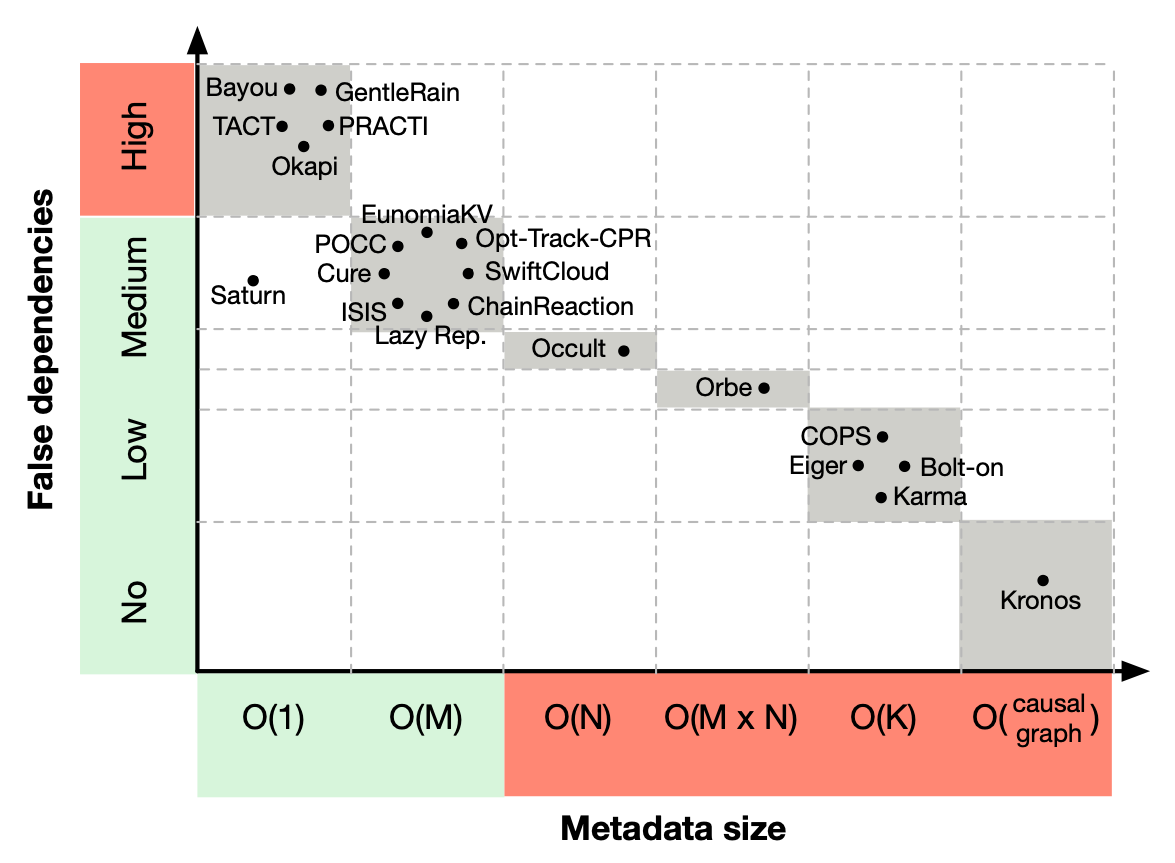
\includegraphics[scale=0.3]{figures/soa-metadata-graph.png}
    \caption{Graphic distribution of existing causally consistent systems based on the metadata size used to capture causal dependencies and the amount of false dependencies that each solution generates. Colored cells represent the diagonal. M, N, and K refers to the number of datacenters, partitions and keys respectively. Colored in green (lightly colored) and red (darkly colored) the different sizes of metadata and types of false dependencies.}
    \label{fig:soa-metadata-graph}
\end{figure*}

As expected, 
there is a direct correlation between the metadata size and the amount of false 
dependencies, 
which is why most of the solutions stand in the diagonal (colored cells). 
This is due to the fact that, 
in all existing solutions, 
the order in which each datacenter applies remote updates locally must be inferred
exclusively from the metadata. 
Thus, on the one hand, when metadata is aggregated, 
false dependencies induce poor remote visibilities compared to systems tracking 
causality more precisely. 
On the other hand, when metadata is not aggregated, 
the associated computation and storage overhead has an impact in throughput.